\documentclass{article}
\usepackage{times}

% \documentstyle[nips07submit_09,times]{article}

%% Standard packages
\usepackage{color}
\usepackage{graphicx}
\usepackage{subfigure}
\usepackage{rotating}
\usepackage{multirow}
\usepackage{url}
%\usepackage{epsfig}
\usepackage{bm}
\usepackage{bbm}
\usepackage{algorithm}
\usepackage{algorithmic}
\usepackage[compact,small]{titlesec}
\usepackage[accepted]{icml2010stylefiles/icml2010}
%% Math packages
\usepackage{amsmath}
\usepackage{amsfonts}
\usepackage{mathrsfs}
\usepackage{bm}
\usepackage{wrapfig}
\usepackage{natbib}

% \log\def\comment#1{}
\newcommand{\fix}{\marginpar{FIX}}
\newcommand{\new}{\marginpar{NEW}}
%% Common macros
%\newcommand{\expectsub}[2]{\mathbb{E}_{#1}\left[#2\right]}
\newcommand{\expect}[1]{\expectsub{q}{#1}}
\newcommand{\entropy}[1]{\mathrm{H}(#1)}
\newcommand{\KL}[2]{\mathrm{KL}(#1 || #2)}
\newcommand{\covariates}{\mathbf{\psi}(\topicmean_{d},\topicmean_{d'})}
\newcommand{\ecovariates}{\overline{\mathbf{\psi}}_{d,d'}}
\newcommand{\myeq}[1]{Equation~\ref{#1}}
\newcommand{\mysec}[1]{Section~\ref{#1}}
\newcommand{\logit}{\mathrm{logit}}
%\newcommand{\invlogit}{\logit^{-1}}
\newcommand{\invlogit}{\sigma}
\newcommand{\partialphi}{\frac{\partial}{\partial\phi_{d,j}}}
\newcommand{\partialphil}{\frac{\partial}{\partial\phi_{d,j,l}}}
\newcommand{\partialeta}{\frac{\partial}{\partial\bm{\eta}}}
\newcommand{\partialnu}{\frac{\partial}{\partial\nu}}
\newcommand{\myfig}[1]{Figure~\ref{#1}}
\newcommand{\mytable}[1]{Table~\ref{#1}}

\newcommand{\regressionparams}{\bm{\eta}, \nu}
\newcommand{\topicmean}{\overline{\mathbf{z}}}
\newcommand{\vtopicmean}{\overline{\mathbf{\phi}}}
\newcommand{\topicproportion}{\theta}
\newcommand{\transpose}[1]{#1^{\mathrm{T}}}
\newcommand{\Dir}{\mathrm{Dir}}
\newcommand{\Mult}{\mathrm{Mult}}
\newcommand{\DP}{\mathrm{DP}}
\newcommand{\GEM}{\mathrm{GEM}}
\newcommand{\Var}{\mathrm{Var}}

\newcommand{\todo}[1]{{\bf TODO: #1}}

%% added by dave
\newcommand{\g}{\, | \,}
\newcommand{\myeq}[1]{Equation~\ref{eq:#1}}
\newcommand{\mysec}[1]{Section~\ref{sec:#1}}
\newcommand{\myfig}[1]{Figure~\ref{fig:#1}}

%\pagestyle{fancy}

%% Name macros
\newcommand{\mv}{\tilde{m}} 
\newcommand{\z}{\bold{z}} 
\newcommand{\vv}[0]{\tilde{V}}
\newcommand{\W}{\textbf{W}}
\newcommand{\w}{\textbf{w}}
\newcommand{\vphi}{\phi}
\newcommand{\bv}{\tilde{\beta}}
\newcommand{\bb}{\beta}
\newcommand{\ellv}{\tilde{\ell}}
\newcommand{\vlv}{\sigma^2_{\ell}}
\newcommand{\vd}{\sigma^2_{d}}
\newcommand{\vbv}{\sigma^2}
\newcommand{\diag}[1]{\mbox{Diag}\left( #1 \right)}
\newcommand{\stdnorm}[1]{\mathcal{N}\left(#1\right)}

\newcommand{\tr}[0]{\mbox{Tr}}
% \newcommand{\expect}[1]{\mathbb{E}\left[#1\right]}
\newcommand{\expectq}[1]{\mathbb{E}_q\left[#1\right]}
\newcommand{\expectqnoarg}[0]{\mathbb{E}_q}
\newcommand{\defn}[0]{:=}
\newcommand{\partl}[2]{\frac{\partial #1}{\partial #2}}

% \usepackage[small]{caption} 


\newenvironment{packed_enum}{
  \begin{enumerate}
    \setlength{\topsep}{1pt}
    \setlength{\itemsep}{2pt}
    \setlength{\parskip}{1pt}
    \setlength{\parsep}{1pt}
}{\end{enumerate}}


                                        % Helps LaTeX put figures where YOU want
\renewcommand{\topfraction}{0.9}        % 90% of page top can be a float
\renewcommand{\bottomfraction}{0.9}     % 90% of page bottom can be a float
\renewcommand{\textfraction}{0.1}       % only 10% of page must to be text

% The \author macro works with any number of authors. There are two commands
% used to separate the names and addresses of multiple authors: \And and \AND.
%
% Using \And between authors leaves it to \LaTeX{} to determine where to break
% the lines. Using \AND forces a linebreak at that point. So, if \LaTeX{}
% puts 3 of 4 authors names on the first line, and the last on the second
% line, try using \AND instead of \And before the third author name.
%% 
%% TODO for this paper:
%% 1. Update equations, for \beta
%% 2. Determine log likelihood
%% 2. Implement
%% 
%% Experiments
%% 1. Citations
%% 2. Predictive likelihood of data.
%% 3. Held-out perplexity
%% 2. Metric:
%%   Average increase in topic words vs. document weights
%%     - 5, 
%% 3. Run this over 3 corpora:
%%   - Nature
%%   - ACL anthology
%%   - recommendation by Drago
%%   - resource.org
%% 4. 

\icmltitlerunning{Measuring Article Influence Without Citations}

\begin{document}

%\cfoot{ Submitted to ICML 2010.  Please do not redistribute. }
%\cfoot{ Submitted to ICML 2010.  Please do not redistribute. }
%\renewcommand{\footrulewidth}{20pt}

\twocolumn[
\icmltitle{Measuring Article Influence Without Citations}
\icmlauthor{Sean M. Gerrish}{sgerrish@cs.princeton.edu}
%\icmladdress{Department of Computer Science, Princeton University,
%  35 Olden St., Princeton, NJ 08544 USA}
\icmlauthor{David M. Blei}{blei@cs.princeton.edu}
\icmladdress{Department of Computer Science, Princeton University,
  35 Olden St., Princeton, NJ 08544 USA}

\icmlkeywords{influence,impact factor,latent dirichlet
  allocation,dynamic topic model,bibliometrics,unsupervised}
\vskip 0.2in
]


\begin{abstract}
Identifying the most influential documents in a corpus is an important
problem in many fields, from information science and
historiography to text summarization and news aggregation.
Unfortunately, traditional bibliometrics such as citations are often
not available.  We propose using changes in the thematic content of
documents over time to measure the importance of individual documents
within the collection.  We describe a dynamic topic model for both
quantifying and qualifying the impact of these documents and validate
this model empirically.
\end{abstract}

\label{chapter:influence}

A fundamental problem in research and industry is that of organizing
collections of documents.  In many cases this problem can be reduced
to identifying those documents which have been the most influential.
This is an important and common problem in many fields, including
research in academic fields such as political science, history, and
science.  Influence measurements are used to assess the quality of
academic instruments, such as journals, scientists, and universities;
as such, they can play a role in decisions surrounding publishing and
funding. These measurements are critical for academic researchers:
finding and reading the influential articles of a field is central to
good research practice.

Measurements of influence are also significant in industry, as
regulations such as Sarbanes Oxley require public companies to retain
documents.  E-discovery is another field in which identifying
influential documents is critical.  A recent New York Times article
cited the need for such tools in industry:
\begin{quote}
  \emph{``The economic impact will be huge,'' said Tom Mitchell, chairman
    of the machine learning department at Carnegie Mellon University
    in Pittsburgh. ``We're at the beginning of a 10-year period where
    we're going to transition from computers that can't understand
    language to a point where computers can understand quite a bit
    about language.''} \citep{markoff:2011}.
\end{quote}
The article continues, noting that recent solutions use either
keyword-based search methods or take advantage of metadata such as
citations or links in emails, which can be helpful when available.
Metadata can be a boon for finding the most influential documents in a
collection, but often such metadata is unavailable.

In this chapter, we will describe an approach to identifying
influential articles in a collection without the use of metadata like
citations.  The key assumption of our method is that an influential
article will affect how future articles are written and that this
effect can be detected by examining the way corpus statistics change
over time.  We will take advantage of the tools discussed in the last
chapter by using them to encode this intuition in a model to measure
influence in sequential collections of documents.

\subsection*{Measuring influence with citations}

A traditional method of assessing an article's influence is to count
the citations to it. The impact factor of a journal, for example, is
based on aggregate citation counts~\citep{garfield:2002}.  This is
intuitive: if more people have cited an article, then more people have
read it, and it is likely to have had more impact on its field.
Citation counts are used with other types of documents as well.  The
Pagerank algorithm, for example, uses hyperlinks of web-pages to
identify the most influential Webpages on the Internet, and it was
essential to Google's early success in Web search~\citep{brin:1998}.
There is a large literature on these and other methods for citation
analysis and bibliometrics.  See~\cite{osareh:1996} for a review.

Though citation counts can be powerful, they can be hard to use in
practice.  Some collections, such as news stories, blog posts, or
legal documents, contain articles that were influential on others but
lack explicit citations between them.  Other collections, like OCR
scans of historical scientific literature, do contain citations, but
they are difficult to read in reliable electronic form.  Finally,
citation counts only capture one kind of influence.  All citations
from an article are counted equally in an impact factor, when some
articles of a bibliography might have influenced the authors more than
others.

\subsection*{Using text to measure influence}

One possible solution might be to \emph{predict} citation counts, by
proposing features and training a regression. \cite{tang:2009} and
\cite{lokker:2008} have used methods like this; successful features include
the publishing journal's impact factor, previous citations to last
author, key terms, and number of authors
\citep{tang:2009,lokker:2008}.  Such research has had measured
success: 56\% explained variance \citep{lokker:2008}, and 91.5\%
prediction accuracy \citep{ibanez:2009}.

However, we seek a model that is applicable to collections for which
the notion of citation may not exist.  Therefore, predicting citations
is an explicit non-goal.  Further, work toward predicting citations
uses specialized classifiers and restrictive features for narrow
application domains; \cite{lokker:2008} even note that their results
``may not be readily transferable to... basic science articles or
journals''. They further noted that earlier work in their field of
predicting citations to medical journals had only achieved 14\% to
20\% explained variance \citep{lokker:2008}.

%\subsubsection*{Using text to measure influence}

%interdisciplinary journal such as \textit{Nature} might have influence
%on Neuroscience without having influence on Genomics.  In our model,
%both the topics and influential articles are inferred.

In this chapter we will use a text-based approach to measure influence.
We will base our assumptions on a topic model which allows topics to drift
over time in a corpus~\citep{blei:2006}. Though our algorithm aims to
capture something different from citation, we will validate the
inferred influence measurements by comparing them to citation counts.

We begin with a discussion of previous work aimed at modeling
influential documents.  We then describe the Document Influence Model
(DIM), our unsupervised model for determining the influence of a
document using the changes in language used by documents over time.
We follow this with experiments to compare this model with citation
counts on three well-known scientific corpora and a collection of
legal opinions.  We will also provide the reader with an intuition for
the model with several real-world examples. With only the language of
the articles as input, our algorithm produces a meaningful measure of
each document's influence in the corpus.

\section{The Document Influence Model}
\label{section:model}

In this section we will develop a probabilistic model that captures
how past articles exhibit varying influence on future articles.  The
hypothesis is that an article's influence on the future is
corroborated by how the language of its field changes subsequent to
its publication.  In the model, the influence of each article is
encoded as a hidden variable; the posterior distribution of these
variables (given the text of documents) reveals the influential articles
of the collection.

\subsection*{Past approaches}
A number of algorithms link the text of documents to citation counts.
This work often models the information in citations by predicting them
or modeling them with
topics~\citep{nallapati:2008,chang:2009,dietz:2007,Cohn01themissing} or
other semantic tools \citep{mcnee:2002,ibanez:2009}.  Other work in
this area uses the text of documents along with citations to summarize
documents \citep{qazvinian:2008} or to propose new bibliometrics:
\cite{mann:2006} use topic models and citations to map topics over
time and define several new bibliometric measurements such as topic
Impact Factor, topical diffusion, and topic longevity.

Some work in this area uses the link structure of citation networks to
extract higher level structure. \cite{borner:2003}, for
example, have used author and citation networks to understand the
evolution of ideas in the history of science.

\subsection*{Dynamic Topics}
\begin{figure}
  \centering
  \begin{tabular}{cc}
    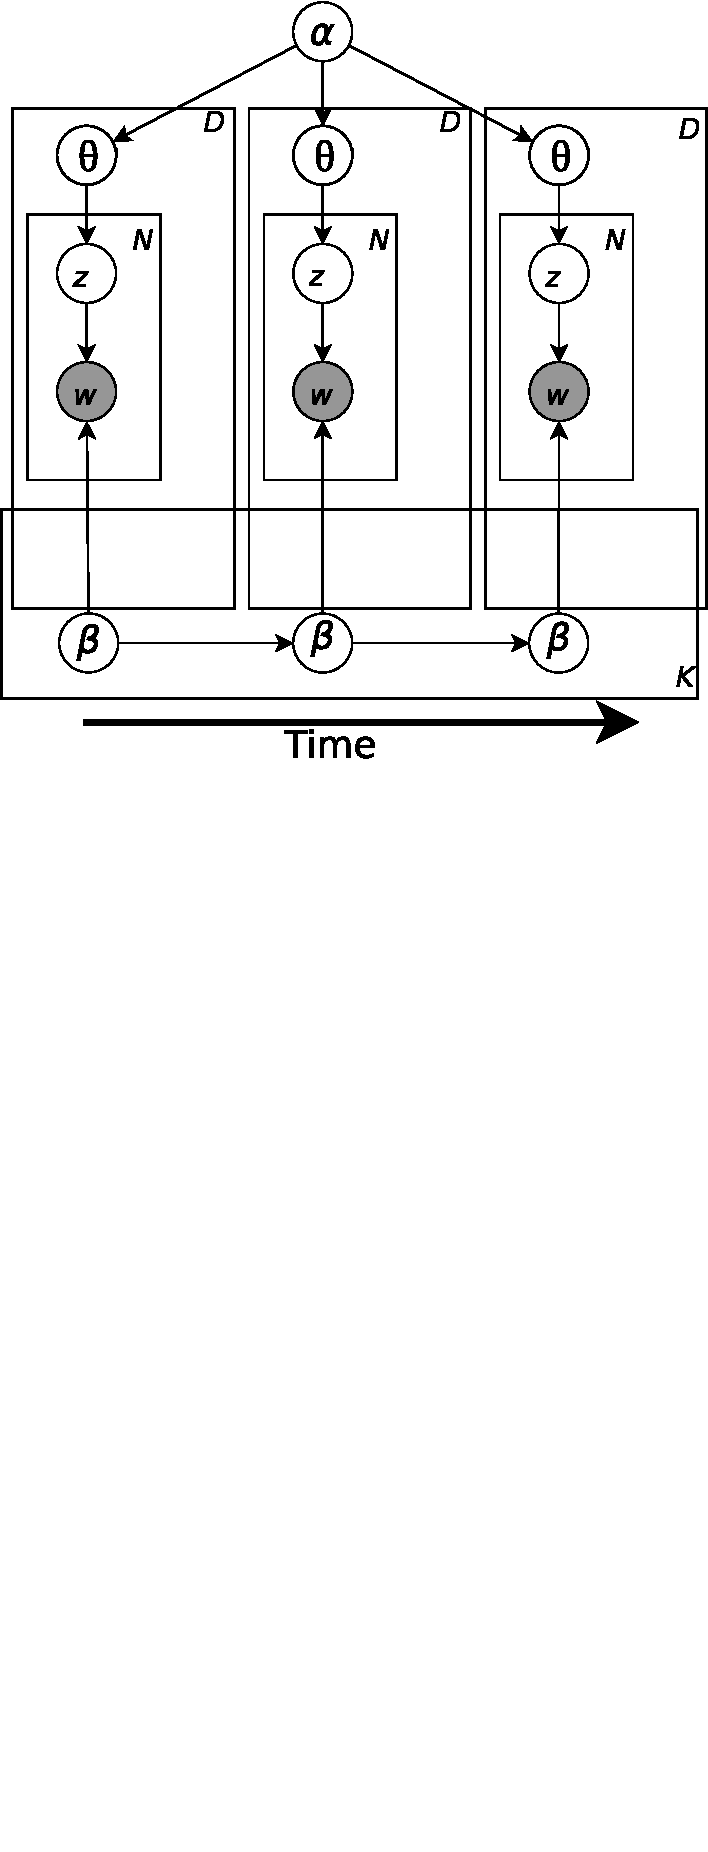
\includegraphics[width=0.3\textwidth,bb=50 500 350 800]{chapter_influence/figures/dtm_gm.pdf} &
    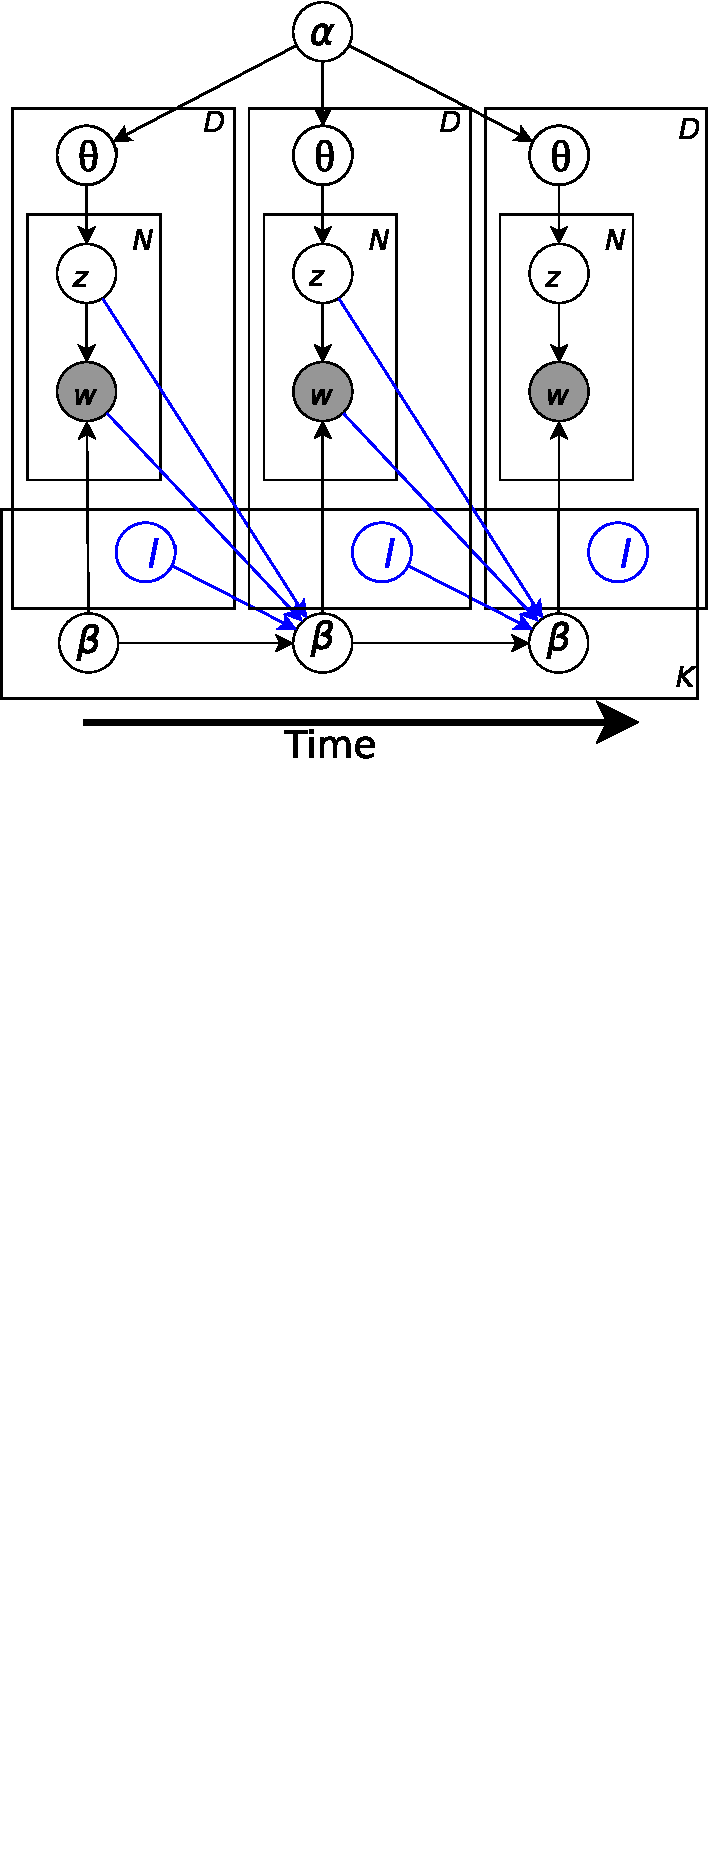
\includegraphics[width=0.3\textwidth,bb=-50 500 250 800]{chapter_influence/figures/docinf_gm.pdf} \\
    (a) & (b) \\
  \end{tabular}
 \label{fig:doc_influence_model}
  \caption{\label{fig:gm} The Dynamic Topic Model (a) and the the Document Influence Model (b).}
\end{figure}

Our model is based on the dynamic topic model (DTM)~\citep{blei:2006},
a model of sequential corpora that allows language statistics to drift
over time.  Probabilistic topic models such as LDA (introduced in the
last chapter) usually assume that the underlying distribution over
words is fixed \citep{blei:2003,deerwester:1990,hofmann:1999}. The DTM
introduced a Markov chain of term distributions to capture
probabilities that drift over the course of the collection.  The idea
is simple: topics drift in discrete steps over time.  At each
``epoch'', some number of documents are generated based on topics \emph{at that epoch}.

\paragraph{Drifting Topics.} We can formalize these assumptions in a
statistical model as in \cite{blei:2006}.  First let
$V$ be the number of words in a vocabulary and consider the natural
parameters $\beta_t$ of a term distribution at time $t$, where the
probability of a word $w$ is given by the softmax transformation of
the unconstrained vector,
\begin{equation}
  \label{eq:softmax}
  p(w \g \beta_{t}) \propto \exp(\beta_{t,w}).
\end{equation}
The corresponding distribution over terms, i.e., the ``topic,'' is a
point on the vocabulary simplex.  In the logistic normal Markov chain,
this distribution drifts with the stationary Markov process
\begin{equation}
  \label{eq:logistic-normal}
  \beta_{t+1} \g \beta_t \sim \mathcal{N}(\beta_{t}, \sigma^2 I),
\end{equation}
where $\sigma^2$ is the transition variance. 
% In the simplest DTM, a
% single distribution over words drifts according to
% \myeq{logistic-normal}.

\paragraph{Documents generated at time $t$.} Now consider a corpus
broken up into discrete epochs $t \in \{ 1, \ldots, T \}$, with $D_t$
articles at each time $t$.  Let $\W_{t,1:D}$ denote the articles as
vectors of word counts, where row $\w_{t,d}$ of $\W_{t, 1:D}$
represents the word counts in article $d$.

At each epoch $t$, the documents of these articles are drawn independently
using the topics described by \myeq{softmax}.  More formally, documents
are generated according to the generative model
\begin{enumerate}
\item For time $t=1, \ldots, T$:
  \begin{enumerate}
  \item For topics $k=1, \ldots, K$:
    \begin{enumerate}
    \item Draw topics $\beta_{k,t} \g \beta_{k,t-1} \sim \mathcal{N}(\beta_{k,t}, \sigma^2 I)$
    \end{enumerate}
  \item For document $d=1, \ldots, D_t$:
    \begin{enumerate}
    \item Draw topic mixture $\theta_d \sim \mbox{Dir}(\alpha, \ldots, \alpha)$.
    \item For term $n=1, \ldots, N$:
      \begin{enumerate}
      \item Draw topic indicator $z_n \sim \mbox{Mult}(\theta_d)$.
      \item Draw word $w_n$ according to \myeq{softmax}.
      \end{enumerate}
    \end{enumerate}
  \end{enumerate}
\end{enumerate}

We illustrate the graphical model for in \myfig{doc_influence_model} (a). With this
model in hand and a collection of documents, one can then estimate the
positions of these topics by computing the posterior distribution of
the sequence of topics $\beta_{1:T}$ conditioned on the observed
documents.  This summarizes the corpus as a smooth trajectory of word
frequencies.

\subsection*{The Document Influence Model}
We now turn to the original problem: certain ideas are influential in
the progression of a field, and we aim to discover what these ideas
are (as doing so will allow us to find those documents are
influential).  The text of documents will provide a window into these
underlying patterns.

In our model, each article is assigned a normally distributed
\textit{influence score} $\ell_d$, which is a scalar value that
describes the influence that article $d$ has on the topic.  The higher
the influence, the more the words of the article affect how the topic
drifts.

This is encoded in the time series model.  The more influential a
document is, the more its words ``nudge'' the topic's natural
parameters at the next time step,
\begin{equation}
  \begin{split}
    \label{eq:logistic-normal-influence}
    \beta_{t+1} \g & \beta_t, (w, \ell)_{t,1:D} \sim
    \mathcal{N}\left(
      \beta_{t} +
      \exp(-\beta_t) \sum_d w_{d,t} \ell_{t,d},
      \sigma^2 I
    \right).
  \end{split}
\end{equation}
The words of an article with a high influence will have a higher
expected probability in the next epoch; the words of an article
with zero influence will not affect the next epoch.

% smg: Do you think the reader will understand the role of this term?
% The $\exp(-\beta_t)$ term makes influence meaningful in the space of
% natural parameters.

We call this model the \textit{document influence model}
(DIM). Conditioned on a corpus, the posterior distribution of the
topic and influence scores gives a trajectory of term frequencies and
a retrospective estimate of the influence of each article.  An article
whose words can help explain the way the word frequencies change will
have a high posterior influence score.  We will show in \mysec{results}
that this estimate of influence is meaningful.

\paragraph{Multiple topics.}  Corpora typically contain multiple
persistent themes.  Accordingly, the full dynamic topic model contains
multiple topics, each associated with a time series of distributions.
Conditioned on the topics, articles at each time are modeled
with latent Dirichlet allocation (LDA).  Each article exhibits the
topics with different random proportions $\theta_d$; each word of each
article is drawn by choosing a topic assignment from those proportions
$z_{d,n}$, and choosing a word from the corresponding topic
~\citep{blei:2003}.

Modeling multiple topics is important to the influence model because
an article might have different impact in the different fields that it
discusses.  For example, an article about computational genomics may
be very important to biology but less important to computer science.
We want to discern its influence on each of these topics separately.

As with the DTM, we posit $K$ topic trajectories, and each document of
each time point is modeled with LDA.  For each document, we now
associate an influence score $\ell_{d,k}$ for each topic $k$.  Each of
the $K$ topics drifts according to an adapted version of
\myeq{logistic-normal}, where we restrict attention to the influence
score for that topic and to the words of each document that were
assigned to it,
\begin{equation}
  \begin{split}
    \label{eq:logistic-normal-influence-topics}
    \beta_{k,t+1} & \g \beta_{k,t}, (w, \ell, z)_{t,1:D} \sim
    \mathcal{N}\left(
      \beta_{k,t} +
      \exp(-\beta_{k,t}) \sum_{d} \ell_{d,k} \sum_n w_{d,n} z_{d,n,k},
      \sigma^2 I
    \right).
  \end{split}
\end{equation}
Here, $z_{d,n,k}$ is the indicator that the $n$th word in document $d$
is assigned to topic $k$ and we have dropped the index $t$ on $z$ and
$w$.  The graphical model is illustrated \myfig{gm} (b).

Although we presented our model in this section with influence
spanning one year, we also adapted it to accomodate an ``influence
envelope'', where an article's influence spans $W$ years.  This
provides a more realistic model of influence \citep{porter:2005}, but
it complicates the inference algorithm and may not be necessary, as we
note in section~\ref{sec:results}.

% dmb: do we name the model anywhere as the DIM?
% smg: this is noted earlier (I think you added it in your rev.).

To use this model, we analyze a corpus through posterior inference.
This reveals a set of $K$ changing topics and influence scores for
each article and each topic.  The posterior provides a thematic window
into the corpus and can help identify which articles most contributed
to the development of its themes.

\subsection*{Work with similar goals}

It is worth pointing out two pieces of recent research have similar
goals. \cite{leskovec:2009} describe a framework for tracking the
spread of memes, or ideas, in document collections, and investigate
the direction in which ideas tend to percolate.
\cite{shaparenko:2007} describe a measure of influence by modeling
documents as unigram mixtures of earlier documents and use a
likelihood ratio test to predict citations between documents. In
contrast to this work, the DIM uses dynamic topics to explicitly model
the change in \emph{topic} language.  Further, we do not attempt to
model links between documents, as in \cite{shaparenko:2007}.  % citet

\section{Inference and parameter estimation}
\label{section:inference}

Our computational challenge is to compute the posterior distribution
of the latent variables---the sequences of topics and the per-document
influence values---conditioned on observed documents in the corpus.
As for simpler topic models, this posterior is intractable to compute
exactly. We therefore employ variational methods---introduced in
Chapter 2---to fit this posterior.

To apply variational methods, we begin by specifying a variational
distribution for the DIM posterior.  First, the word assignments $z_n$
and topic proportions $\theta_d$ are governed by multinomial
parameters $\phi_d$ and Dirichlet parameters $\gamma_d$, as in
LDA~\citep{blei:2003}; we refer to these distributions as $q(z_n |
\phi_n)$ and $q(\theta_d | \gamma_d)$.

The variational distribution for topic trajectories
$\{\beta_{k,1}, \ldots, \beta_{k,T} \}$ is described by a linear
Gaussian chain.  It is governed by parameters $\{ \bv_{k,1}, \ldots,
\bv_{k,T} \}$, which are interpreted as the ``variational
observations'' of the chain.  These induce a sequence of means $\mv_t$
and variances $\vv_t$. \cite{blei:2006} call this a ``variational
Kalman filter.''

Finally, the variational distribution of the document influence value
$\ell_{d,k}$ is a Gaussian with mean $\ellv_{d,k}$ and fixed variance
$\vlv$.
% ~\footnote{In general, we may abuse notation and refer to the
%  vector $\ellv_{t,k}$ of all document weights at time $t$ for topic
%  $k$; notation should be evident from context.}

% dmb: above, do we fit the variance term or is it fixed?  (in the
% influence variational distribution)
% smg: I've kept the variance term fixed.

% dmb: above, do we really need that footnote?
% smg: if you think it's unnecessary, then probably not.

% dmb: below, do we ever say that "x" is all the latent variables?  do
% we really need this shorthand?
% smg: I can try to 

In full, the variational distribution is
\begin{align}
  q(\beta, \ell, z, \theta | & \bv, \ellv, \phi, \gamma) = \prod_{k=1}^K q(\beta_{k,1:T} | \bv_{k,1:T})
  \prod_{t=1}^T \prod_{d=1}^{D_t} q(\theta_{t,d} | \gamma_{t,d})
  q(\ell_{d} | \ellv_{d})
  \prod_{n=1}^{N_{t,d}} q(z_{t,d,n} | \vphi_{t,d,n}). \nonumber
\end{align}
% dmb: use different notation from d... it looks like the document index
% smg: that's what d is -- which d are you referring to?
% dmb: in general, clean up this equation.  i'm not sure you need the
% first integral.  it suffices to go right to the terms.  and, i think
% that multiple sums will look better than parentheses.
Using this variational family, our goal is to maximize the Evidence Lower Bound (ELBO) $\mathcal{L}$ on the model evidence of the observed words $\W$:
\begin{align}
  \label{eq:elbo}
  \ln p(\W) \geq & \mathcal{L}(\bv, \vphi, \gamma) \\
  = & \sum_T \expectq{\ln p(\beta_{t} | \beta_{t-1})} 
  + \sum_{T} \sum_{D_t} \expectq{\ln p(\ell_{d})} + \expectq{\ln
    p(\theta_{d} | \alpha)} \label{eq:elbo_line2} \\ 
  & + \sum_{T} \sum_{D_t} \sum_{N_d} \expectq{\ln p( z_n | \theta_d)} + \expectq{\ln p(w_n | z_n, \beta_t)}
  + H(q). \label{eq:elbo_line3}
\end{align}
Note also that the variational parameters $\bv, \vphi,$ and $\gamma$
are implicit in lines~\ref{eq:elbo_line2} and~\ref{eq:elbo_line3} of
the above equation because they parameterize the variational
distribution $q$, and the expectation is taken with respect to this distribution.

\subsection*{Optimizing the variational bound}
This bound is optimized by variational EM, with an update schedule similar to that in \cite{blei:2006}:
\begin{enumerate}
\item For Topic $k=1, \ldots, K$:
  \begin{enumerate}
  \item Update parameters $\bv_k$.
  \end{enumerate}
\item For time $t = 1, \ldots, T$:
  \begin{enumerate}
  \item For document $d_{1,t}, \ldots, d_{{D_t}, t}$:
    \begin{enumerate}
    \item Update parameters $\vphi_d$, and $\gamma_d$
      \end{enumerate}
    \item Update parameters $\ellv_t$ (i.e., update $\ellv_d$ as a
      block for all documents at time $t$),
    \end{enumerate}
  \end{enumerate}    
where the variational parameters are optimized sequentially in
blocks.  These updates are repeated until the relative increase in
the lower bound is below a threshold (we specify this in the
experiments section).

\paragraph{Topic trajectories.}
The variational update for $\bv$ is similar to that in
\cite{blei:2006}. For each topic, we update the variational Kalman   % citet
``observations'' by applying gradient ascent:
\begin{align*}
\partl{\mathcal{L}}{\bv_{sw}} =
% From beta generative rule:
   & -  \frac{1}{\sigma^2} \sum_{t=1}^T
     \left( \mv_{tw} - \mv_{t-1,w} - G_{t-1,w} \right) 
      \left( \partl{\mv_{tw}}{\bv_{sw}}
     - \partl{\mv_{t-1,w}}{\bv_{sw}}
     + G_{t-1,w} \partl{\mv_{t-1,w}}{\bv_{sw}} \right) \\
   & +  \sum_T \left(
       N_{w,t} - N_{t} \zeta_t^{-1}
       \exp( \hat{m}_{\bb_{tw}} + \frac{\tilde{V}_{tw}}{2} ) \right)
       \partl{\mv_{tw}}{\bv_{sw}}  \\
    & +  \frac{1}{\sigma^2} \sum_{t=1}^T
         \partl{\mv_{t-1,w}}{\bv_{sw}}
         \left( H_{t-1,w} - G_{t-1,w}^2 \right) 
    +  \frac{1}{\sigma^2} \sum_{t=0}^{T-1}
         \partl{\mv_{tw}}{\bv_{sw}}
         G_{tw} \vv_{tw},
\end{align*}
where
\begin{eqnarray*}
%\mbox{where} \\
 G_{sn} &=& \expectq{\exp(-\beta_{s,k,n} ) ( \W_{s,k,n} \circ
  z_{s,k,n} ) \ell_{s,k}} \\
 H_{sn} &=& \mathbb{E}_q \big[ \exp(-2 \beta_{s,k,n}) \left( (\W_{s,k,n} \circ z_{s,k,n} ) \ell_{s,k} \right)^2 \big].
\end{eqnarray*}

Note also that we have added the additional variational parameter
$\zeta_t$ and the term $\partl{\mv_{tn}}{\bv_{sn}}$, which are both
described in \cite{blei:2006}. The % citet
former can be updated once per iteration with $\zeta_t \gets \sum_w
\exp(\mv_{t,n} + \vv_{t,n}/2)$. The latter can be derived from the
variational Kalman filter updates (see \myapp{docinf_appendix} and
\cite{blei:2006}).

\paragraph{Influence values.}
In the DIM, changes in a topic's mean parameters are governed by a
normal distribution.  As a consequence of this choice, updates for the
influence parameters $\ellv_{t,k}$ solve a linear regression.  In this
regression, documents' words at time $t$ explain the expected topic
drift $\bm{\Delta_{\beta,t,k}} = (\beta_{t+1,k} - \beta_{t,k})$, where
the contributions of each document's words are given by the design
matrix $X = \diag{\exp(-\beta_{t,k})} (\bm W_{t,k} \circ \phi_{t,k}
)$. ($\diag{\vec{x}}$ refers to the matrix having the elements of
$\vec{x}$ on its diagonal.)
%\begin{eqnarray}
%\bm{\Delta_{\beta,t,k,w}} := & \hspace{-34pt} \exp(-\mv_{t,k,w} + \vv_{t,k,w} / 2) \nonumber \\
%& \hspace{-11pt} \times \hspace{2pt} (\mv_{t+1,k,w} - \mv_{t,k,w} + \vv_{t,k,w}). \nonumber
%\end{eqnarray}

The parameter updates for document influence $\ellv_{t,k}$ are
defined, for each time $t$ and each topic $k$, by the
variational normal equation
\begin{align}
\ellv_{t, k} \gets \big(  \frac{\vbv}{\vd} \bm I
  + \expectq{X^T X} \big)^{-1} \expectq{X^T \bm{\Delta_{\beta,t,k}}}.
  \label{eq:regression}
\end{align}
%\begin{align*}
%\[ \small
%\bm H_{t,k} = \expectq{(\bm W_t \circ z_{t,k})^T \diag{\exp(-2\beta_{t,k})} (\bm W_t \circ z_{t,k})}; \\
%\normalsize
% & 
% (\bm W_{t,k} \circ \vphi_{t,k})^T \diag{h_{\exp}}
%   (\bm W_{t,k} \circ \vphi_{t,k}) \nonumber \\
% & \hspace{-25pt}  + \mbox{Diag} \Big( (\bm W_{t,k} \circ \bm W_{t,k} \circ ( \vphi_{t,k} - \vphi_{t,k} \circ \vphi_{t,k}))^T h_{\exp} \Big), \nonumber \\
%\end{align*}
%\]
The expectation $\expectq{X^TX}$ is a matrix with dimension $D_t \times D_t$.  Its elements are
\begin{eqnarray*}
 {\expectq{X^T X}}_{d,d'} = \sum_n \exp(-2\mv_{t,k,n} + 2 \vv_{t,k,n}) (w_{t,d,n} w_{t,d',n} \phi_{t,k,d,n } \phi_{t,k,d',n})
\end{eqnarray*}
when $d \neq d'$ and
\begin{eqnarray*}
{\expectq{X^T X}}_{d,d} = \sum_n \exp(-2\mv_{t,k,n} + 2 \vv_{t,k,n}) (w_{t,d,n}^2 \phi_{t,k,d,n})
\end{eqnarray*}
otherwise. The expectation $\expectq{X^T \bm{\Delta_{\beta,t,k}}}$
is a $D_t$-dimensional matrix with elements
\begin{eqnarray*}
 {\expectq{X^T \bm{\Delta_{\beta,t,k}}}}_d = 
 \sum_n & \hspace{-10pt} w_{t,d,n} \phi_{t,k,d,n} 
  \times (\mv_{t+1,k,n} - \mv_{t,k,n} + \vv_{t,k,n}/2) 
  \times \exp(-\mv_{t,k,n} + \vv_{t,k,n}/2). 
\end{eqnarray*}

\paragraph{Topic proportions and topic assignments.}
Updates for the variational Dirichlet on the topic proportions
$\theta_{d,k}$ have a closed-form solution, exactly as in LDA
\citep{blei:2003}; we omit details here.

The variational parameter for each word $w_n$'s hidden topic $z_n$ is
the multinomial $\phi_n$.  We solve for $\phi_{n,k}$ by the
closed-form updates
\begin{align}
\label{eq:phi_update}
%\log(\phi_{w,k}) & \gets & \Psi(\gamma_k) + \mv_{t, k,w} \nonumber \\
%& & \hspace{-60pt} + \frac{1}{\sigma^2} \bm w_{t} \ellv_{d_w,k} \big( \exp(-\mv_{t,k,w} + \vv_{t,k,w} / 2) \nonumber \\
%    & & \hspace{-10pt} \times  (\mv_{t + 1,k,w} - \mv_{t,k,w} + \vv_{t,k,w}) \big) \nonumber \\
%   & & \hspace{-60pt} - \frac{1}{\sigma^2} \bm w_{t} \exp(-2 \mv_{t} + 2 \vv_t) \big( 
%        \ellv_{d} \times (\bm W_t \circ \phi_{t,k}^{\mbox{L}} \ellv_{t,k})_w \nonumber \\
%   & & \hspace{55pt} + \bm w_{t} \phi_{w,k}^{\mbox{L}} \ellv_{d}^2 - \ellv_{d}^2 - \sigma_l^2 \big) \nonumber \\
\log(\phi_{n,k}) \gets & \Psi(\gamma_k) + \mv_{t,k,n} + \frac{1}{\sigma^2} w_{t} \ellv_{d_n,k} \exp(-\mv_{t,k} \hspace{-1pt} + \hspace{-1pt} \vv_{t,k} / 2) (\mv_{t+1,k} - \mv_{t,k} + \vv_{t,k})  \nonumber \\ 
& - \frac{1}{\sigma^2} w_{t,n} \Big[ \ellv_{d_n,k} \exp(-2\mv_{t,k} + 2 \vv_{t,k})
 (\bm W_{t,n,\setminus{d_n}} \circ \phi_{t,n,k,\setminus{d_n}}) \ellv_{t,k,\setminus d_n} \Big] \nonumber \\
& - \frac{1}{\sigma^2} w_{t,n}^2 \exp(-2\mv_{t,k} + 2 \vv_{t,k}) (\ellv_{d,n,k}^2 + \sigma_l^2),
\end{align}
where $\Psi$ is the digamma function and $\setminus{d_n}$ refers to
the set of all documents \emph{except} $d_n$. Solving the constrained
optimization problem, this update is followed by normalization
$\phi_{w, k} \gets \frac{\phi_{w, k}}{\sum_K \phi_{n, k}}$.

\section{Empirical study}

We studied three collections of scientific articles and a collection
of opinions written by judges in the New York Appellate Court system.
For each corpus, we estimated and examined the posterior distributions
of its articles' influence.

In this section, we demonstrate that the estimate of an article's
influence is robustly correlated to the number of citations it
received.  While the DIM model is designed for corpora without
citations---and, indeed, only the documents' text and dates are used
in fitting the model---citations remain an established measure of
influence.  This study provides validation of the DIM as an
exploratory tool of influential articles.

% dmb: not an svn error: i re-added the sentence above.  i liked it.

% We also provide several examples to demonstrate that this model
% provides a bibliometric similar to citations with distinctive
% qualities.

\subsection*{Data}
\label{sec:data}

% dmb: put this fact somewhere else.  did inference take the same
% amount of time for each corpus?

% smg: it was close, with nature taking a little longer.  I don't know
% where else it belongs, so I'll leave it out.

% dmb: well, it's nice to give an example of how long inference takes.
% i think it's okay to say something like "to give a sense for how
% long the algorithm takes, the XXX corpus with XXX topics took XXX
% time to converge on an XXX machine."  also, i suggest briefly adding
% details like the variational convergence criterion and how the model
% is initialized.  (no need to report sensitivity, just give the facts
% so that someone can replicate our experiments.)

% smg: re-added, below.
% 

The three scientific corpora we analyzed were the \emph{ACL
  Anthology}, \emph{The Proceedings of the National Academy of
  Science}, and the journal \emph{Nature}.  For each corpus, we
removed short documents, terms that occurred in too few documents, and
terms that occurred in too many documents.  We also removed terms
whose statistics did not vary over the course of the collection, as
such terms would not be useful for assessing change in language (a
sample of such non-varying terms from \emph{Nature} is ``ordinarily'',
``shake'', ``centimetre'', ``traffic'', and ``themselves'').

\textbf{ACL Anthology.} The \emph{Association for Computational
  Linguistics Anthology} is a digital collection of publications about
computational linguistics and natural language
processing~\cite{bird:2008}.  We analyzed a 50\% sample from this
anthology, spanning 1964 to 2002.  Our sample contains 7,561
articles and 11,763 unique terms after preprocessing.  For this corpus
we used article citation counts from the \emph{ACL Anthology
  Network}~\cite{Radev:2009}.

\textbf{PNAS.} The \emph{Proceedings of the National Academy of
  Sciences} is a leading, highly-cited, multidisciplinary scientific
journal covering biological, physical, and social sciences.  We
sampled one seventh of the collection, spanning 1914 (when it was
founded) to 2004.  Our sample contains 12,145 articles and 14,504
distinct terms after preprocessing.  We found citations using Google
Scholar for 78\% of this collection.

\textbf{Nature.} The journal \emph{Nature} is the world's most highly
cited interdisciplinary science journal~\cite{Thompson:2009} with
content on a range of scientific fields. We analyzed a $10\%$
sample from this corpus, spanning 1869 (when it was founded) to
2008.  Our sample contains 34,418 articles and 6,125 distinct terms
after preprocessing.  We found citations using Google Scholar for 31\%
of these documents.

% smg: Note that this will make us run out of space.
Inference for 10 topics on each corpus above took about 11 hours to
converge on a desktop Intel 2.4GHz Core 2 Quad cpu.  Our convergence
criterion was met when the evidence lower bound increased by no more
than 0.01\%.  For the experiments described below, we set topics'
Markov chain variance $\sigma^2=0.005$ and $\sigma_d=\sigma_l=0.0001$.


% \begin{figure}
%  \small
% \begin{centering}
%   \caption{Preprocessing thresholds for each corpus.}
%   \begin{tabular}{|l|l|l|l|}
%     \hline
%     Minimum fraction of documents & 0.2\% & 0.4\% & 0.3\% \\
%     Maximum fraction of documents & 25\% & 15\% & 20\% \\
%     Maximum fraction of documents &      &      &      \\
%     in any year & 40\%& 30\% & 40\% \\
%     Minimum stdandard deviation & 0.75 & 1.2 & 1.5 \\
%     \hline
%     & \emph{Nature} & \emph{PNAS} & \emph{ACL} \\
%     \hline
%   \end{tabular}
%   \label{fig:preprocess_thresholds}
%   \end{centering}
%   \normalsize
%     \vspace{-10pt} \\
% \end{figure}

\subsection*{Relating posterior influence and citation}
\label{sec:results}

We studied the DIM with varying numbers of topics.  We measured the
relationship between the posterior influence values of each article
$\ellv_d$ and its citation count $c_d$.

We first aggregate the influence values across topics.  Recall that
each document has an influence value for each topic.  For each word,
we compute its expected posterior influence score, with the
expectation taken with respect to its (random) topic assignment.  We
then sum these values over all words in the document,
\begin{equation}
  f(\ellv_d) = \sum_{n=1}^{N_d} \textrm{E}[z_{d,n} \cdot \ellv_d].
  \label{eq:score}
\end{equation}
This weights each word by the influence associated with its assigned
topic.  (Using the maximum value of influence across topics yielded
similar results.)

% dmb: below, i commented out this paragraph.  this seemed like it
% shouldn't be there anymore since you added a part about the new
% metric.  that said, perhaps you should add a point about taking
% correlation to log, if that is still what we're doing.

% \paragraph{Metrics.}  We used two metrics to measure the relationship
% between the aggregated influence scores and citations.  First, we
% computed the correlation between influence score and $\log(c_d + 1)$,
% which provides a commonly understood test statistic.  We take the log
% to account for overdispersion---once an article is cited, it is likely
% to be cited more.  We also 

%Second, we compute a metric, the standardized median deviation, on the
%first fifty most influential articles.  (Our idea is that this is a
%reasonable number for a scientist to examine.)  First, we standardize
%the log citations, computing for each article the number of standard
%deviations from the mean of the log citations.  This step is taken to
%make this metric comparable across datasets that have different
%numbers of citations.  We then select the top 50 documents $\{
%d_{i_1}, \ldots, d_{i_{50}} \}$ by their aggregate posterior influence
%and compute the median standardized citation of them.  This provides a
%robust indication of the model's performance on its top documents; the
%typical article will have value 0, and a bad article will have a
%negative value.

% dmb: has the idea of the influence envelope been added to the
% modeling section?  it should be...

% smg: Yes, I moved it there in the earlier revision.

% \paragraph{Influence envelope}
% One might expect that documents tend to have greatest influence
% shortly after publishing; indeed, the median number of citations to
% scientific articles begins decreasing within 10 years
% \cite{porter:2005}.  One parameter in the model determines the amount
% of influence an article has after $n$ years
% \begin{align*}
%   \textstyle r_n(t) = \left\{
%     \begin{array}{ll}
%       \frac{1}{n} & t <= n  \\
%       0 & t >= n
%     \end{array} \right., t = 0, 1, 2, \ldots,
% \end{align*}
% where we refer to $r_n$ as the \emph{influence envelope} of length $n$. While
% this envelope is discontinuous and arguably unnatural, it remains
% simple and provides useful information about the model. Across all
% corpora, we found that shorter envelopes yield a closer
% relationship between our model and citations.

\begin{figure*}[t]
  \centering
  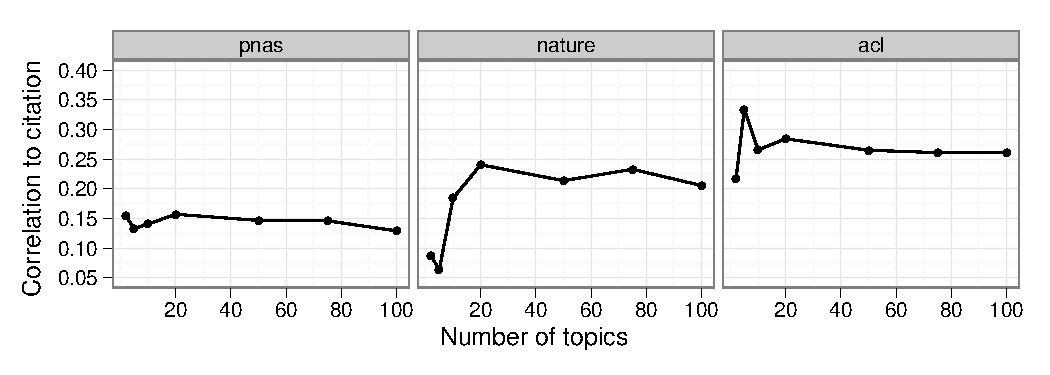
\includegraphics[width=0.8\textwidth]{chapter_influence/figures/results_correlation.pdf} \\
  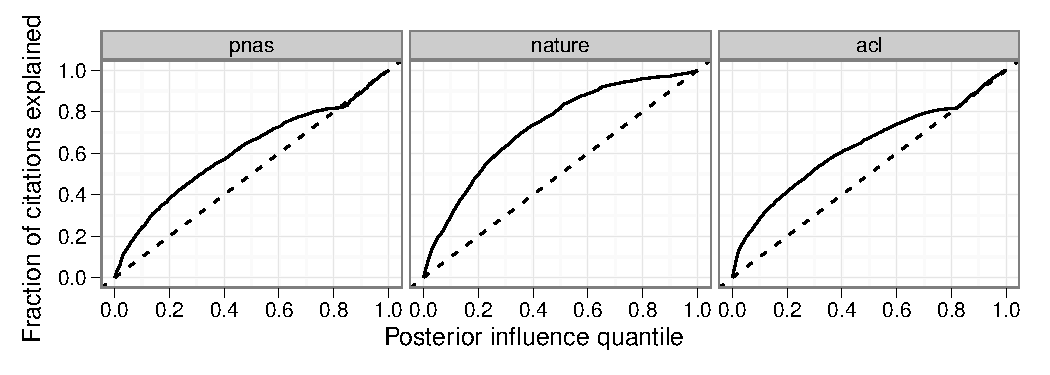
\includegraphics[width=0.8\textwidth]{chapter_influence/figures/results_roc.pdf} \\
  \caption{Spearman rank correlation between citation counts and
    posterior influence score, controlling for date (top) and fraction
    of citations explained by posterior influence (bottom).}
  \label{fig:results}
\end{figure*}

\myfig{results} displays the Spearman rank correlation between the
aggregated posterior influence score of \myeq{score} and citation
counts.  The DIM posterior---which is estimated only from the texts of
the articles---has a positive correlation to the number of citations.
All of these numbers were found significant up to $p<1e-4$, using
permutation tests on the influence scores.

Correlation goes up when we model multiple topics within a corpus.
Moving from 2 to 5 topics in the \emph{ACL} corpus increases
correlation from 0.25 to 0.37.  \emph{Nature} is likewise better with
more topics, with a correlation of 0.28 at 20 topics; while
\emph{PNAS} performs best near 5 topics, with a correlation of 0.20.

% These numbers make sense: the \emph{ACL} corpus is much more
% specialized than \emph{Nature}, so more topics are required to
% discriminate research fields for Nature.

\myfig{results} also shows the fraction of citations explained
by DIM scores: \emph{Nature} documents with the highest 20\% of
posterior influence, for example, received 56\% of citations.  The
flat regions in \emph{ACL} and \emph{PNAS} are due to aggregate
influence scores very close to zero.

% dmb: see my comment above: has the idea of the influence envelope
% been added to the modeling section?
% smg: It should be (provided that there wasn't an svn issue)

% All numbers reported above and plotted use flat influence envelopes of
% 4 years for each of \emph{ACL} and \emph{PNAS} and 10 years for
% \emph{Nature}. We found empirically that small windows of influence
% are most highly correlated with citations, suggesting that the added
% complexity of the larger windows may not be justified.

% dmb: this feels like too much detail.  if a reviewer asks about it,
% we can mention it.  did we end up with random restarts?

% smg: for most of the data, it was random.  for the last set of
% experiments (not included), it wsa not.

% Selecting the correct number of topics is important for the model
% because it defines the granularity at which the model identifies
% influence.  Further, different topics may be found when topics are
% initialized with different random seeds. That said, we still find
% high correlation in results with different initializations and
% differing numbers of topics.  In a 50-topic model vs. a 75-topic
% model over \emph{Nature}, for example, the correlation coefficient
% of documents' posterior influence is 0.72.

\paragraph{Heuristic model.} 
 The DIM is a complicated model. To
justify its complexity, we describe a simple baseline (the
\emph{heuristic}) which captures our intuition with a single topic, is
easy to implement, and runs quickly.  For this heuristic, we define a
word's weight at time $t$ as:
\[
w_t := \textstyle \frac{\mbox{Frequency of } w \mbox{ in } [t, t + f] }
{\mbox{Frequency of }w \mbox{ in }[t - p, t]
},
\]
for fixed distances $f$ into the future and $p$ into the past.
A document's score is the weighted average of its words'
weights. This heuristic captures the intuition that influential
documents use language adopted by other documents.

% dmb: i'm confused which results are being reported below.  first we
% say that "the model with a single topic generally outperforms the
% heuristic."  then we say "however" the heuristic performs well with
% large values of the parameters.

The heuristic performed best with large values of its parameters
($f=p=200$). With these settings, it achieves a correlation of 0.20 for
the \emph{ACL}, 0.20 for \emph{PNAS}, and 0.26 for \emph{Nature}.  For
\emph{Nature}, the model is more correlated with citations than the
heuristic for 20, 50, and 75 topics.  Correlation is matched for
\emph{PNAS}, the model slightly beating the heuristic at 5 topics.
\emph{ACL} outperforms the heuristic for all numbers of topics.

\paragraph{Shuffled corpus} Though we have eliminated date as a
confounder by controlling for it in correlations, there may be other
confounders such as document length or topic distribution.  We
therefore measured the DIM's relationship to citations when dates were
randomly shuffled, keeping all documents which share a date
together. If non-date confounders exist, then we might see correlation
in the shuffled data, marking observed correlation as dubious.

We shuffled dates in the corpora and refit the DIM.  We found a
\emph{maximum} date-controlled correlation of 0.018 for 29 shuffles of
\emph{ACL}; 0.001 for 5 shuffles of \emph{Nature}; and 0.012 for 28
shuffles of \emph{PNAS}. While this shuffled experiment and
controlling for date do not entirely preclude confounding, they eliminate many
potential confounders.

\subsection*{A closer look}
Experiments showing correlation with citations demonstrate consistency
with existing bibliometrics. However, the DIM also finds qualitatively
different articles than citation counts. In this section we describe
several documents to give the reader an intuition behind the kind of
analysis that the DIM provides.

\paragraph{IBM Model 3} The second-most cited article in the \emph{ACL
  Anthology Network} is \emph{The Mathematics of Statistical Machine
  Translation: Parameter Estimation}~\cite{brown:1993}. It has 450
intra-\emph{ACL} citations and 2,130 total citations listed on Google
Scholar.  This seminal work describes parameter estimation for five
word-based statistical models of machine translation; it provided
widely accepted statistical models for word alignment and introduced
the well-known ``IBM models'' for machine translation. The posterior
influence score for \cite{brown:1993} ranked $6$ out of 7,561   %  citet
articles in a 10-topic model.

%Figure~\ref{fig:topics} (top) shows a topic discovered by the DIM
%in which \cite{brown:1993} was the most influential over 40 years:
This article was most influential in a topic about translation, which
had a trend toward ``alignment for machine translation.''  The
largest-moving words are shown in \myfig{words} (left).
Upward trends for ``alignment'', ``brown'', and ``equation'' are
evident (although it is not clear whether ``brown'' refers to the
author or the corpus).

% dmb: below, how many intra-acl citations are there?
\paragraph{The Penn Treebank}
The most-cited article in our subset of the \emph{ACL Anthology
  Network} is \emph{Building a large annotated corpus of English: the
  Penn Treebank} \cite{marcus:1993}, with 1,622 \emph{ACL} citations
and 2,810 citations on Google Scholar.  This article describes the
large-scale part-of-speech and syntax tagging of a 4.5-million word
corpus.  It falls in a topic about part-of-speech tagging and syntax
trees; ``treebank'' had become one of the top words in the topic by
2004.

The DIM assigned a relatively low influence score to this article,
ranking it 2,569 out of 7,561 articles.  While \cite{marcus:1993}  % citet
introduces a powerful \emph{resource}, most of the article uses
conventional language and ideas to detail the annotation of the Penn
Treebank.  As such, the paper does not discuss paradigm-changing ideas
and the model scores it low.  We emphasize that this does not
undermine the tremendous influence that the Penn Treebank has had on
the field of natural language processing.  The DIM is not designed to
discover this kind of influence.

% dmb: below, remind us 1st out of how many articles?
% smg: Added 34,418.
\begin{figure*}
  \center
\normalsize
\begin{tabular}{c}
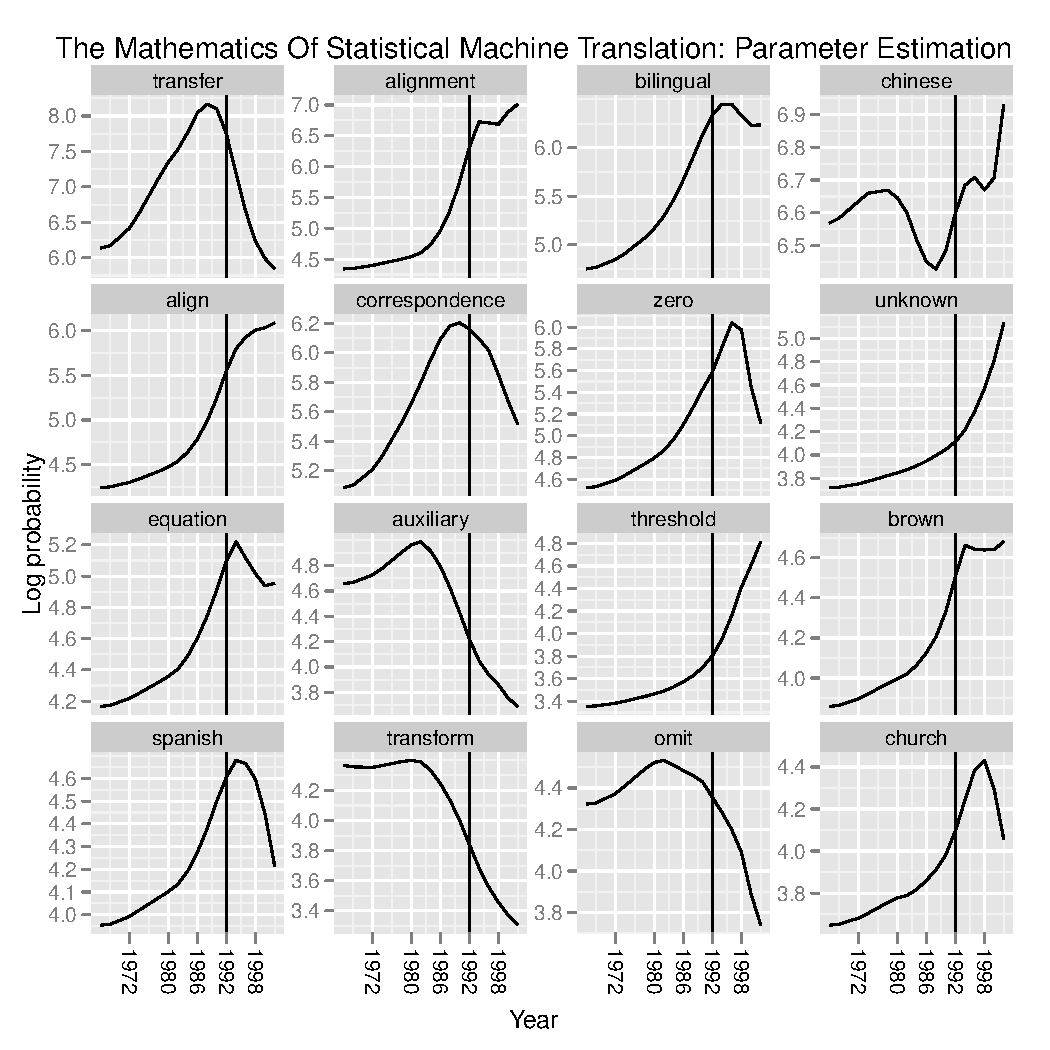
\includegraphics[width=0.7\textwidth]{chapter_influence/figures/acl_brown.pdf}
\\
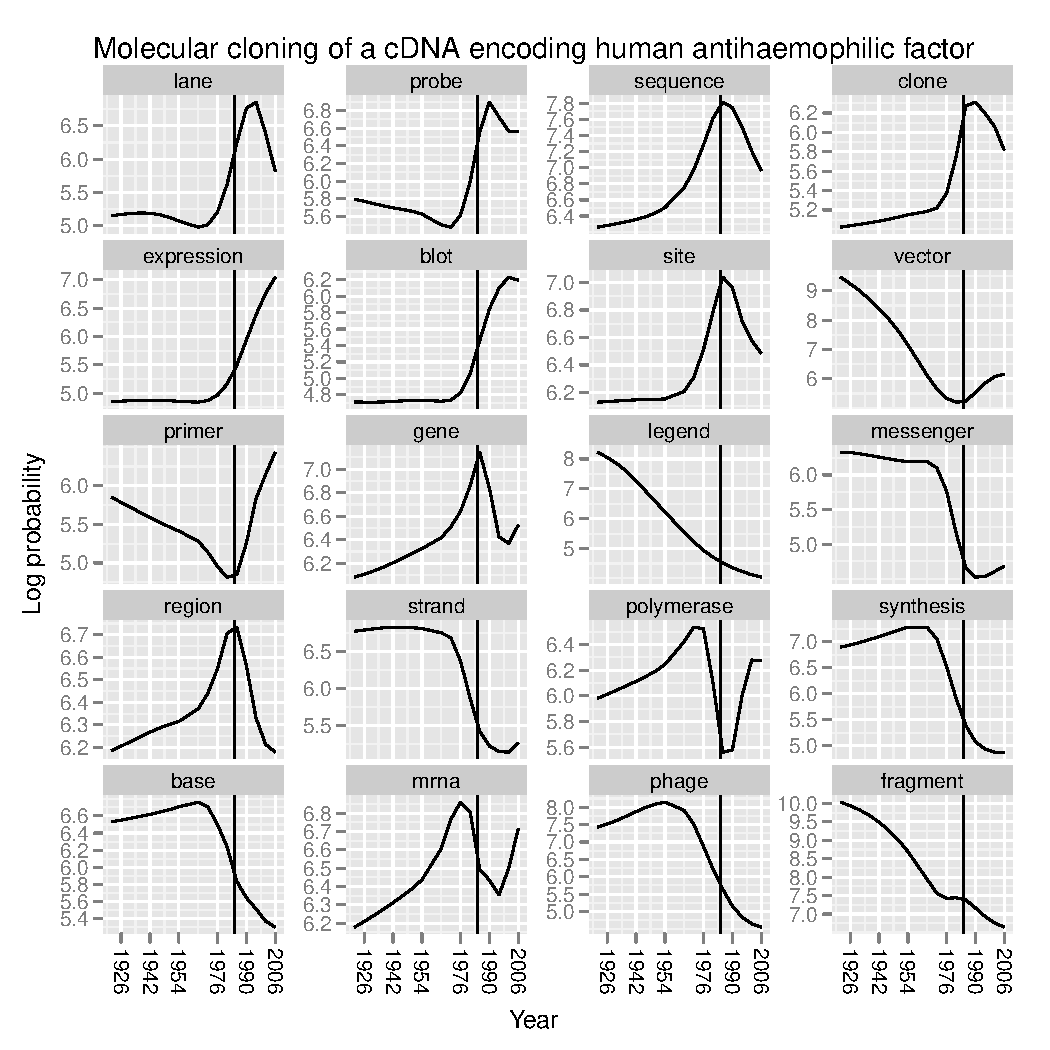
\includegraphics[width=0.7\textwidth]{chapter_influence/figures/nature_cloning.pdf} \\
\end{tabular}
  \small
\caption{Most active words appearing in \cite{brown:1993} (left) which
  have changed the most in a topic about translation. On right are
  words appearing in \cite{toole:1984} in a topic about DNA and
  genetics.  Terms are sorted by increase over 10 years.}  \normalsize
%\label{fig:acl_brown_words}
%\label{fig:nature_cloning}
\label{fig:words}
\end{figure*}

\paragraph{Success in 1972}
In 1967, The College Science Improvement Program was established to
assist predominantly undergraduate institutions.  Two years later
\emph{Nature} published a short column, which has the highest of our
posterior influence in a 20-topic model, out of 34,418 \emph{Nature}
articles.  No citation information was available about this article in
Google Scholar. The column, \emph{How to be Overtaken by Success},
discusses a debate about the ``Miller bill'', which considers funding
for postgraduate education
\cite{Nature.success:1969}. \textit{Overtaken by Success} provides few
research resources to researchers, which may explain lack of citation
information. Instead, it presciently discusses a paradigm shift in a
topic about science, industry, research, and education: ''The record
of the hearings [on the bill] is not merely an indication of the way
the wind is blowing but an important guide to some of the strains
which are now accumulating within the system of higher education...''

In 1972, three years after this article's publication, The NSF
Authorization Act of 1973 made the NSF explicitly responsible for
science education programs \emph{at all levels}
\cite{NSF.website:2010}.  Where this may have been missed by those
using citation counts to study the history of science education, the
DIM has provided a metric with which to gauge interest in the article.

% dmb: again, remind us out of how many articles.
% smg: Done.

\paragraph{Genetics in \emph{Nature}}
The sixth most influential document by the DIM in a 20-topic model of
\emph{Nature} is \emph{Molecular cloning of a cDNA encoding human
  antihaemophilic factor}, an article describing successful
cloning of a human mRNA sequence important in blood clotting
\cite{toole:1984}.  With 584 citations, this article is among the top
0.2\% of these 34,418 documents.  The most active words
appearing in this article are shown in
\myfig{words} (right).  The plot shows some of the
document's key words -- ``expression'', ``primer'', ``blot'' -- become
prominent words in the topic.

\subsection{An application to the New York Appellate Courts.}

The New York Appellate Court system hears appeals cases within the
state of New York.  This court ``was established to articulate
statewide principles of law in the context of deciding particular
lawsuits.''  \cite{nyca_webpage:2012}, acting as a form of ``Supreme
Court'' for the state of New York.  Judges who hear these cases make
decisions about the cases and write opinions summarizing their
reasoning for these decisions.  These decisions and opinions are
extremely important within the court system because they set precedent
for later decisions.

These opinions written by judges are therefore written expressly to be
\emph{influential} on later court decisions, and judges' opinions
frequently make explicit citations to earlier cases.  However, these
citations are limited in two respects.  First, multiple opinions may
exist per case, stating the majority opinion, supporting it in part,
or entirely disagreeing with it. Although judges' citations are
explicit and well-formatted, their citations do not make this
distinction machine-readable making large-scale analyses difficult
without expensive hand-coding. Second, lawmakers may have different
reasons for citing opinions; it has been hypothesized by some
political methodologists that researchers do not cite dissenting
opinions because dissenting opinions are considered to hold little if
any legal sway; citing dissenting opinions is therefore seen as a sign
of weakness \cite{beim:2011}.

We analyzed this collection, splitting xxx appellate court cases into
xxx distinct opinions, written by judges representing the majority
opinion, a concurrance in part (i.e., supporting the majority decision
but with a different rationale for reaching that decision), or a
dissenting opionion.  Our collection contained xxx distinct terms
after pre-processing. We also scraped citations within this collection
and found xxx citations.

We then fit a 40-topic model to this collection to discover
influential documents.  Consistent with the scientific corpora, we
measured a Spearman rank-correlation coefficient between posterior
influence scores and the logarithm of citation counts at $\rho=0.24$.
We illustrate the fraction of citations explained by documents above
different influence thresholds in
\myfig{nyca_citations_explained}.  We also briefly discuss the
results anecdotally below.

\begin{figure}
  \center
  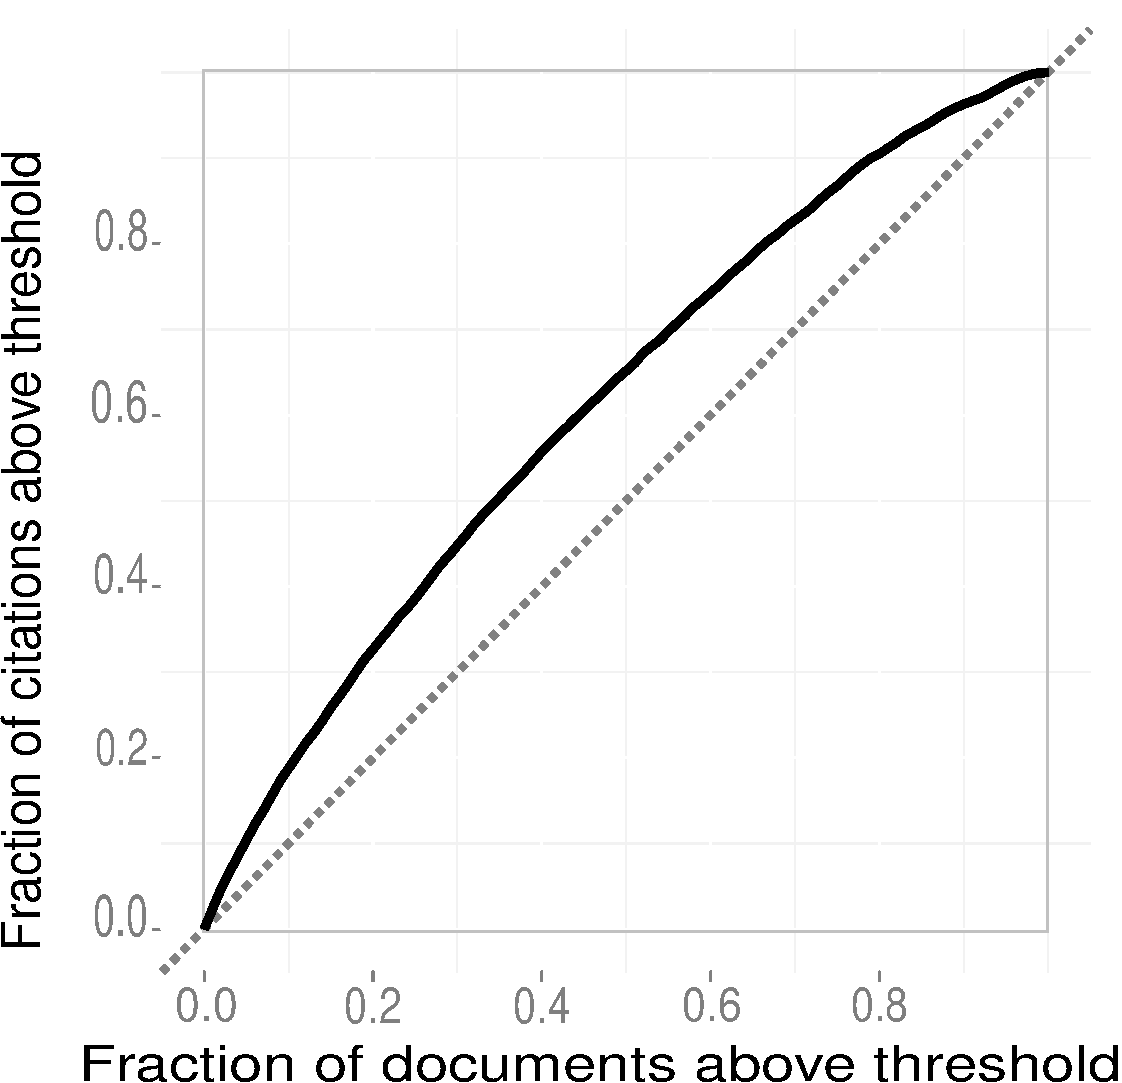
\includegraphics[width=0.4\textwidth]{chapter_influence/figures/fraction_docs_vs_fraction_citations.pdf}
  \caption{Citations explained by influence score in the New York Appellate Courts.  Each point on the curve represents a different threshold of the influence score.  The x-axis describes threshold on the influence score, and the y-axis describes the fraction of citations for all documents which fall below this threshold.}
  \label{fig:nyca_citations_explained}
\end{figure}



\paragraph{The Cardozo Topic.} Judge Benjamin Cardozo (later Justice
Cardozo) was one of the most well-known judges in American political
history.  Cardozo is known for his thoughtful, deliberate opinions and
is considered to have had an outsize influence on judicial thought.
One of the more interesting topics discovered by our model in this
collection identified language which was predominantjuly used by Judge
Benjamin Cardozo.\footnote{A similar topic was discovered by a dynamic
  topic model.}  This topic used phrases such as xxx, xxx, and
xxx. The average ...


% \section{Discussion}

\section{Conclusions}

Traditional bibliometrics like citations are widely used for
understanding collections of text documents.  Much of the past work
for identifying influential documents focuses on measuring or
predicting citations for corpora which have citations.  In this
chapter we described the DIM, which is developed for time-series
corpora without bibliometrics.  We have demonstrated measured
consistency with citations with the model, controlling for confounders
like document length.  However, the information provided by the model
transcends this: the influence score has anecdotally been demonstrated
to provide qualitatively different information than citations.

Based only on the changing statistics of the language in a corpus, we
computed a measure of influence that is significantly related to
observed citation counts. That said, it would be useful to better
understand how this metric is qualitatively different from citations
and other bibliometrics: expert judgment or usage information obtained
from digital libraries might be some avenues.  We leave this for
future work.

We considered several documents evaluated by the model:
\cite{brown:1993} and \cite{toole:1984}, which both had high citations
and high posterior influence; and \cite{marcus:1993}, which had high
citations and low posterior influence.
%posterior influence; and \cite{Nature.success:1969}, which had few or
%no citations and high posterior influence. These examples illustrate
%that the model can produce results
%different from citations which are still interpretable and meaningful
%to researchers: while citation counts often point to resources based
%on new or traditional ideas, the DIM points to articles which discuss
%relatively new ideas more than those which provide specific resources.
These results demonstrate not just that the model is correlated with
citations; it also suggests that the model provides qualitatively
\emph{different} information than citations.

\subsection{Avenues for future work}
The DIM could be made more realistic and more powerful in many ways.
In one variant, individual documents might have their own ``windows''
of influence.  Other improvements may change the way ideas themselves
are represented, e.g. as atomic units, or \emph{memes}
\citep{leskovec:2009}.  Further variants might differently model the
flow of ideas, by modeling topics as birth and death processes, using
latent force models \citep{alvarez:2009}, or by tracking influence
\emph{between} documents, building on the ideas of
\cite{shaparenko:2007} or \cite{dietz:2007}. % citet

We also believe that it would be useful to better understand models like
the DIM in the context of traditional metrics of influence, such as
academic citations, and other metrics of influence, such as usage
data.  Having a better understanding of when this model and
established metrics differ will uncover where our metric may provide
new information that is not yet captured by existing statistics.

\subsection{Next steps}
The work presented in this chapter assumes that the collection of
documents is described by a set of themes, and that these themes
evolve over time.  It describes each document using a mixture over
themes and a vector describing its influence on each of those themes.
This provides a sense of the current of ideas coursing through a
collection of documents.

A limitation of this approach is that it provides too broad a view of
a corpus: it does not provide explicit detail of the underlying story
\emph{within} a collection.  This model describes a corpus as a
collection of topics, and it describes documents as mixtures of themes
and influence weights, but it does not provide any further sense of a
story which changes over time.

In the next chapter we will discuss a model to explore some of these
shortcomings by explicitly modeling the ``story'' within a collection
of text documents.  This approach will use some of the same ideas from
this chapter.  Again we will assume that a collection of text
documents serve as a window into the events within the collection of
historical documents, and again we will encode assumptions by
explicitly modeling them with latent random variables, linked by a
time-series model.  However, by modeling the interactions of entities
within the collection explicitly, and applying posterior inference, we
will learn a story about them.

%\section{Acknowledgements}
%The author would like to thank XXXX XXX, XXX XXX, and XXX XXX for
%their helpful comments, feedback, and proofreading.


\paragraph{Acknowledgements.} We would like to thank the reviewers for their attention to detail and insightful comments.  David Blei is supported by a
Google Research Grant, ONR 175-6343, and NSF CAREER 0745520.

\begin{small}
\bibliographystyle{icml2010stylefiles/icml2010}
\bibliography{../bib}
\end{small}

\end{document}
